\scanpage{34}
\mspage{8}
cas contraire, distinguons deux cas.

a) $H^+=\{1\}$, donc $H\simeq\{1,\sigma\}$, où $\sigma$ est une anti-involution.

1) Si \deleted{\unsure{$\sigma$}} $X^\sigma=\varnothing$, $\sigma$ fixe une métrique sphérique normalisée unique, OK.

2) Si $X^\sigma\ne\varnothing$ i.e. $\sigma$ une inversion, alors le choix d'une métrique sphérique comp. avec $\sigma$ revient à celui d'une paire de pts de $X$ conjugués sous $\sigma$. En particulier, le choix d'un point\inserted{$x$} de $X$ tel que $\sigma x\ne x$ définit une telle métrique sphérique.

b) $H^+\ne\{1\}$. Considérons le\inserted{unique} tore \deleted{\unsure{$T$}} compact de dim $1$ $T$ qui contient $H^+$, et $T.H=N$, ext. de \deleted{\unsure{$\mathbb Z$}} $\mathbb Z/2\mathbb Z$ par $T$. Les éléments \deleted{\unsure{de}} $\sigma$ de $N^-$ fixent $z,z'$, ou les intervertissent, suivant que l'élément $-1$ de $N/T$ opère trivialement sur $T$, ou par symétrie $t\longmapsto t^{-1}$.
\margin{\uline{C'est l'inverse!}}
Dans le premier cas l'ext. $N$ de\inserted{$\gamma=$} $\mathbb Z/2\mathbb Z$ par $T$ est triviale
\[
\left(H^2(\gamma,T)\simeq T^\sigma/N_\sigma(T)=T/T^2\simeq0\right)
\]
dans le deuxième cas on trouve
\[
H^2(\gamma,T)\simeq T^\sigma/N_\sigma(T)\simeq\underbrace{{}_2T}_{\mathbb Z/2\mathbb Z}/0\simeq\mathbb Z/2\mathbb Z.
\]

1) $N$ ext. \uline{centrale} de \deleted{\unsure{$\mathbb Z$}}\inserted{$\gamma$} par $T$, donc $N\simeq T\times\underset{\substack{\Vert\\\{1,\sigma\}}}{\gamma}$ (\unsure{p. direct}) engendré par $T$ et une $\sigma$ \deleted{qui}\inserted{anti-involution} qui \deleted{fixe $z,z'$} intervertit $z,z'$. \deleted{On voit que} \deleted{\unsure{géodésique}}\inserted{\unsure{inversion}} celle-ci est une inversion, \deleted{\unsure{qui}}

\figure{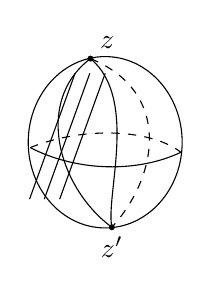
\begin{tikzpicture}[x=.85cm,y=.85cm]
\draw (0,0) ellipse (1.15 and 1.28);
\draw (-.22,1.25) .. controls (-1.08,.6) and (-.68,-.7) .. (.1,-1.27);
\draw (-.22,1.25) .. controls (.5,.65) and (.0,-.8) .. (.1,-1.27);
\draw[dashed] (-.22,1.25) .. controls (1,.75) and (.8,-.5) .. (.1,-1.27);
\draw (-1.12,-.08) .. controls (-.4,-.45) and (.5,-.45) .. (1.13,-.15);
\draw[dashed] (-1.12,-.08) .. controls (-.3,.25) and (.7,.19) .. (1.13,-.15);
\foreach \x in {-.95,-.73,-.5}{\draw (\x-.18,-.85)--(\x+.5,1.03);}
\fill (-.22,1.25) circle (.045) node[above right] {$z$};
\fill (.1,-1.27) circle (.045) node[below] {$z'$};
\end{tikzpicture}}
% archive foliation: 36
